\textcolor{secundario}{DISCOUNT RATE ESTIMATION.} 
The discount rate generally applicable to the estimation of Equity Value can be calculated using financial models known as \gls{wacc} or \gls{wara}. This discount rate consists of the minimum expected return for the organization (\autoref{fig:op_acc} and \ref{fig:narr_val} ).

\begin{figure}[H]
\centering
\begin{minipage}{8cm}
\caption{Opportunity Cost of Shareholders \label{fig:op_acc}}\vspace{5pt}
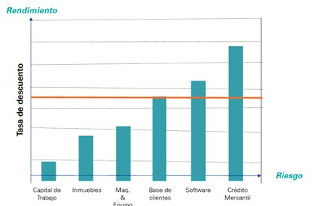
\includegraphics[height=5cm]{\rutaImagenes/costo_oportunidad_accionistas}
\footnotesize{Source: Valuaci\'on de Activos Intangibles. DEAL ADVISORY MEXICO. KPMG C\'ARDENAS DOSAL, S.C. KPMG ``D.R.'' \copyright 2016}
\end{minipage}
\quad
\begin{minipage}{8cm}
\caption{Foundations of Valuation Narrative \label{fig:narr_val}}\vspace{5pt}
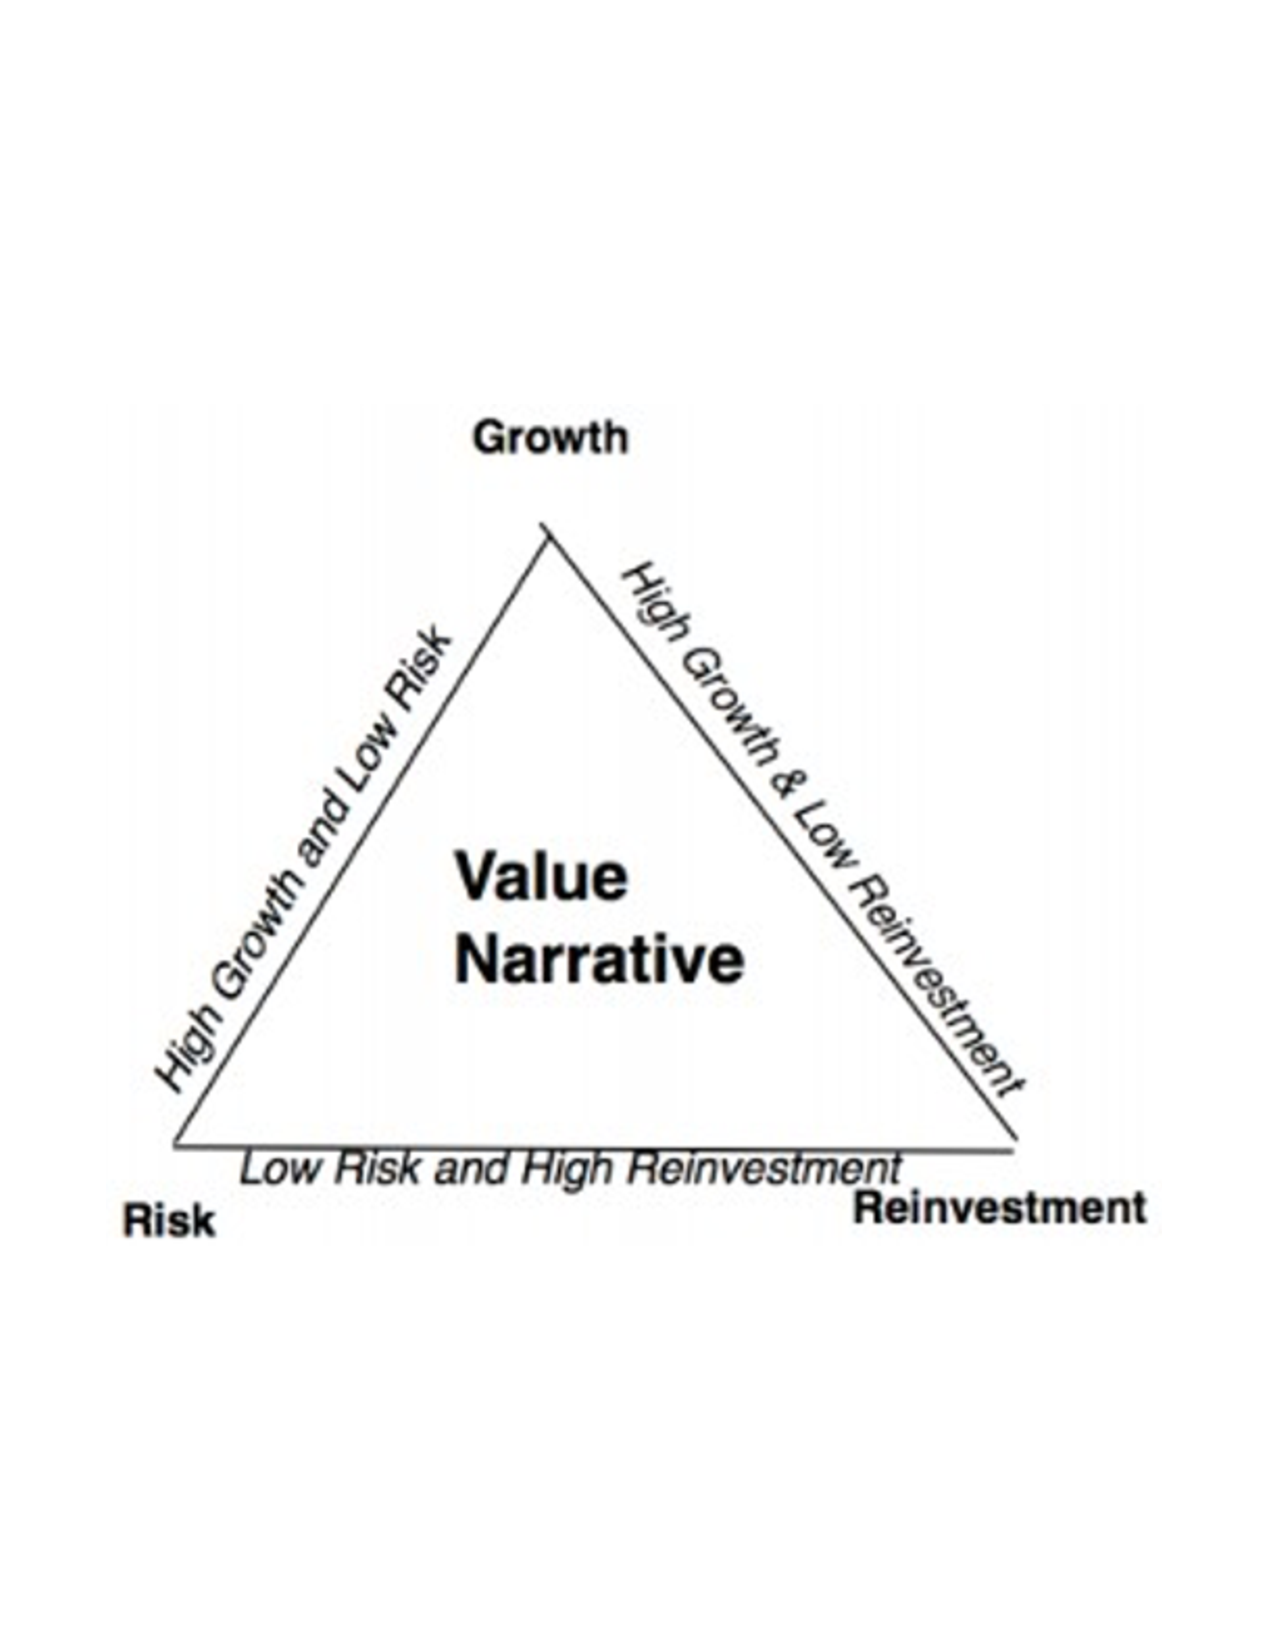
\includegraphics[height=5.5cm]{\rutaImagenes/narrativa_valuatoria}\\
\footnotesize{Source: Damodaran, A. ``Session 14. Narrative to numbers''. NYU/STERN.}

\end{minipage}

\end{figure}

\begin{enumerate}[i)]
\item \textcolor{secundario}{\gls{wacc}} (Weighted Average Cost of Capital). The cost of capital is the compensation that investors demand from firms that use their funds (opportunity cost).
\item \textcolor{secundario}{\gls{wara}} (Weighted Average Return on Assets). Represents the weighted average of the return rates of the Contributory Assets involved in the estimation of the fair value of an  asset.
\end{enumerate}

\begin{figure}[H]
\centering
\caption{Discount Rates WACC \& WARA.\label{fig:wacc_wara}}\vspace{5pt}
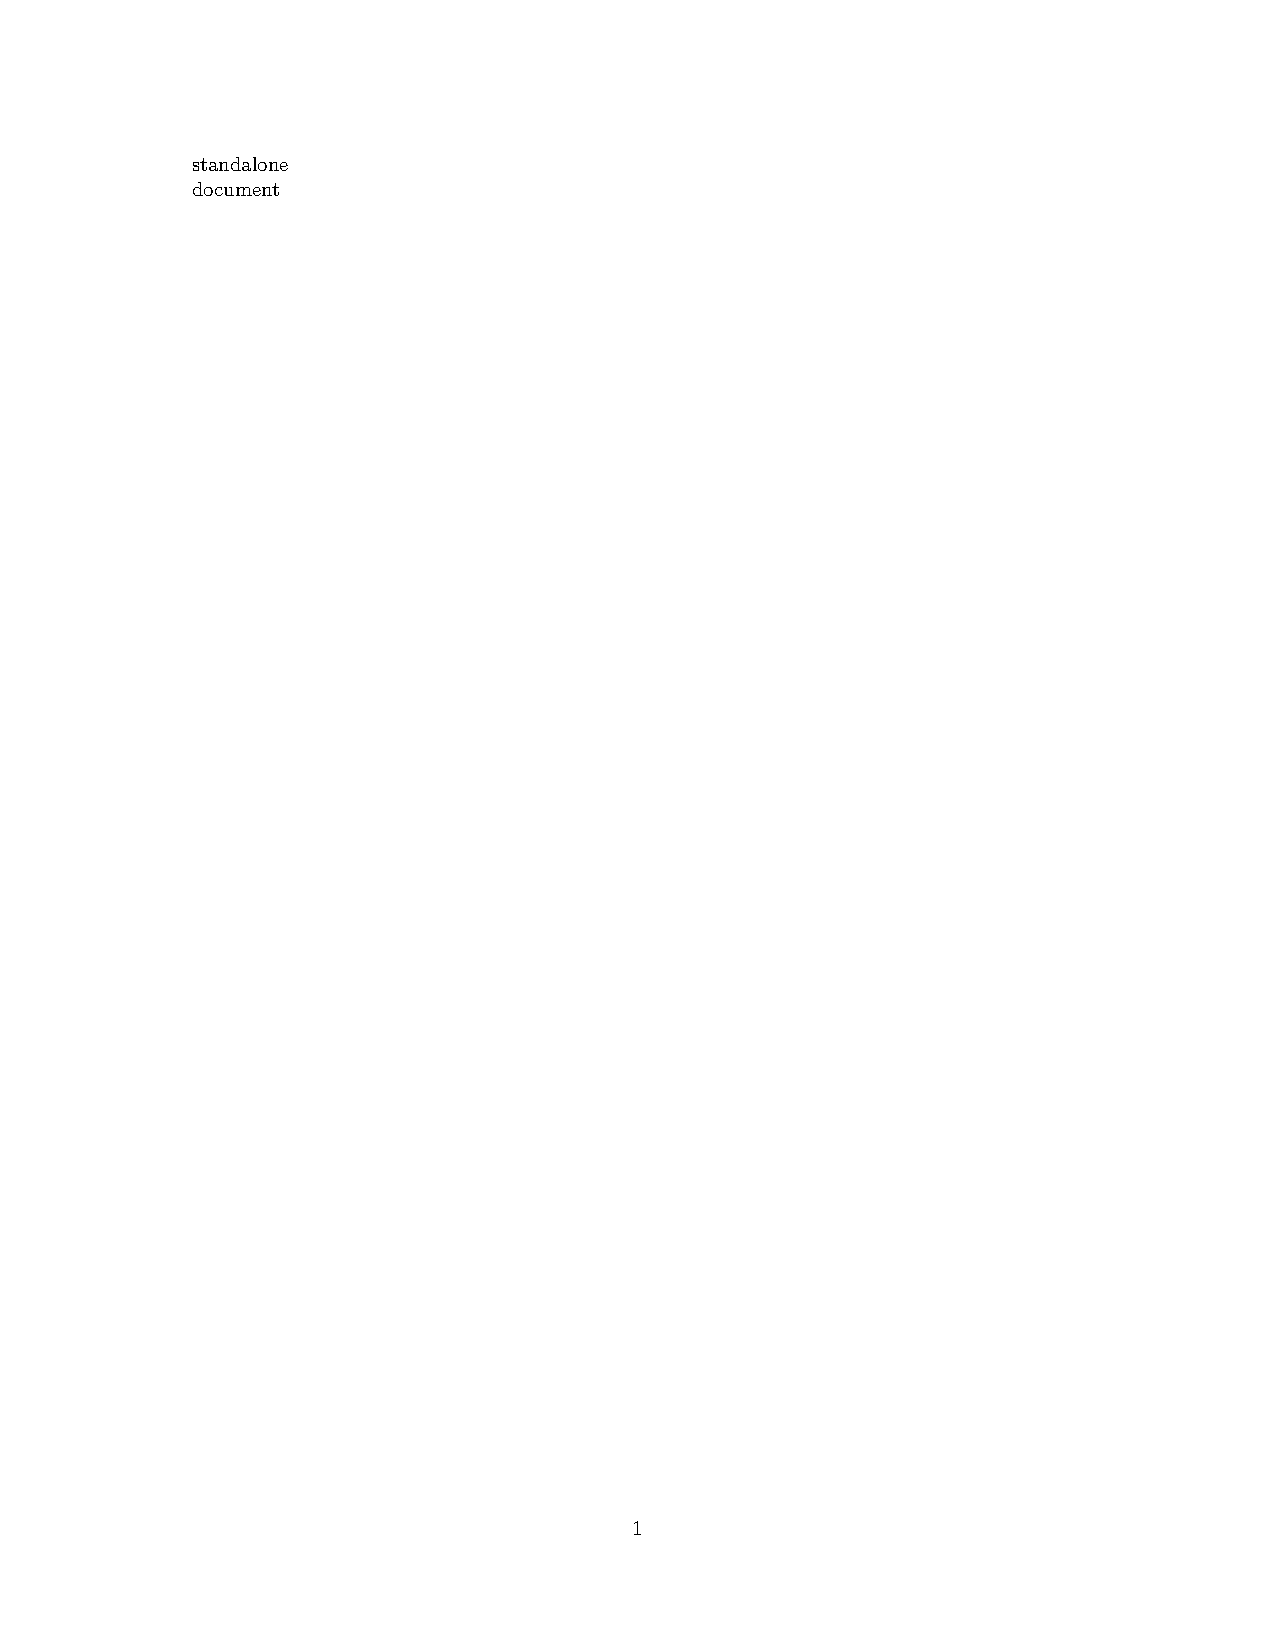
\includegraphics[width=12cm]{\rutaImagenes/wacc_wara}
\end{figure}